
\documentclass[12pt]{article}
\usepackage[english]{babel}
\usepackage[utf8x]{inputenc}
\usepackage{amsmath}
\usepackage{graphicx}
\usepackage[colorinlistoftodos]{todonotes}
\usepackage{caption}
\usepackage{float}
\usepackage{subfig}
\usepackage{comment}
\usepackage{subcaption}
\usepackage{listings}
\usepackage{indentfirst}
\definecolor{codegreen}{rgb}{0,0.6,0}
\definecolor{codegray}{rgb}{0.5,0.5,0.5}
\definecolor{codepurple}{rgb}{0.58,0,0.82}
\definecolor{backcolour}{rgb}{0.95,0.95,0.92}
 \usepackage{tikz}
\usepackage{enumitem}
\usetikzlibrary{trees}
\lstdefinestyle{mystyle}{
    backgroundcolor=\color{backcolour},   
    commentstyle=\color{codegreen},
    keywordstyle=\color{magenta},
    numberstyle=\tiny\color{codegray},
    stringstyle=\color{codepurple},
    basicstyle=\footnotesize,
    breakatwhitespace=false,         
    breaklines=true,                 
    captionpos=b,                    
    keepspaces=true,                 
    numbersep=5pt,                  
    showspaces=false,                
    showstringspaces=false,
    showtabs=false,                  
    tabsize=2
}
\lstset{style=mystyle}
\usepackage{titlesec}
\titleformat{\paragraph}
{\normalfont\normalsize\bfseries}{\theparagraph}{1em}{}
\titlespacing*{\paragraph}
{0pt}{3.25ex plus 1ex minus .2ex}{1.5ex plus .2ex}
\begin{document}


\begin{titlepage}


\newcommand{\HRule}{\rule{\linewidth}{0.5mm}} % Defines a new command for the horizontal lines, change thickness here

\center % Center everything on the page
 
%----------------------------------------------------------------------------------------
%	HEADING SECTIONS
%----------------------------------------------------------------------------------------

\textsc{\LARGE Universidade de Aveiro}\\[1.5cm] % Name of your university/college
\textsc{\Large IEETA}\\[0.5cm] % Major heading such as course name
\textsc{\Large RETIOT}\\[0.5cm]

%----------------------------------------------------------------------------------------
%	TITLE SECTION
%----------------------------------------------------------------------------------------

\HRule \\[0.4cm]
{ \huge \bfseries Technical Report}\\[0.4cm] % Title of your document
\HRule \\[1.5cm]
 
%----------------------------------------------------------------------------------------
%	AUTHOR SECTION
%----------------------------------------------------------------------------------------

\begin{minipage}{0.4\textwidth}
\begin{flushleft} \large
Francisco Santos % Your name
\end{flushleft}
\end{minipage}
~
\begin{minipage}{0.4\textwidth}
\begin{flushright} \large
Nº76618\\
\end{flushright}
\end{minipage}\\[2cm]

% If you don't want a supervisor, uncomment the two lines below and remove the section above
\Large {RETIOT -}
%John \textsc{Smith}\\[3cm] % Your name

%----------------------------------------------------------------------------------------
%	DATE SECTION
%----------------------------------------------------------------------------------------

{\large \emph{February de 2018}}\\[2cm] % Date, change the \today to a set date if you want to be precise

%----------------------------------------------------------------------------------------
%	LOGO SECTION
%----------------------------------------------------------------------------------------


\includegraphics[scale=0.4]{ua_logo.png} % Include a department/university logo - this will require the graphicx package
 
%----------------------------------------------------------------------------------------

\vfill % Fill the rest of the page with whitespace

\end{titlepage}
%%\renewcommand{\figurename}{Figura}
%%\renewcommand{\tablename}{Tabela}
%%\renewcommand{\contentsname}{Conteúdo}
\tableofcontents
\newpage

\section{Introduction}
The focus of this report is to present and explain the various tasks fulfilled in the scope of the project \textbf{RETIOT, “Reflectometry Technologies to Enhance the Future Internet of Things and Cyber-Physical Systems"}. The main objective is to interface the \textit{Texas Instruments mmwave} radar sensor with the \textit{Robot Operating System} and use it to achieve autonomous navigation for the \textbf{turtlebot2} robot.


\section{Procedure}
In order to achieve our objectives the work was split in the following tasks:
\begin{enumerate}
    \item Familiarization with the Robot Operating System architecture and its inner workings.
    \item Create an interface between TI mmwave devices and ROS.
    \item Process the retrieved data in order to  accommodate our application.
    \item Using ROS navigation stack with both radar and lidar sensor information to achieve fully autonomous navigation for the \textbf{turtlebot2} robot.
\end{enumerate}
\section{Robot Operating System}

\subsection{Introduction}
Robot Operating System (ROS) is an open-source, meta-operating system that provides libraries and tools to help developers create robotic applications. This includes hardware abstraction, device drivers, tools for introspection, message-passing and more.
\subsection{ROS architecture}
%MORE STUFF
ROS is composed by:
\begin{itemize}
\item \textbf{Nodes} - Processes that perform computation.
\item \textbf{Messages} - ROS data type used when subscribing or publishing in a topic. 
\item \textbf{Topics} - Nodes can send messages by publishing to a topic or receive them by subscribing to a topic. 
\item \textbf{Master} - Provides registration of names (helps nodes find each other).
% V
\item \textbf{rosout} - ROS equivalent of stdout 
\item \textbf{roscore} - Master+rosout+parameter server. 
%X
\end{itemize}
%%\subsubsection{ROS nodes}
%%\subsubsection{ROS topics}
%%\subsubsection{ROS subscribers and publishers}
%%REVER ISTO
Figure \ref{fig:ros_concepts} shows the general architecture of ROS.

\begin{figure}[!htb]
    \centering
    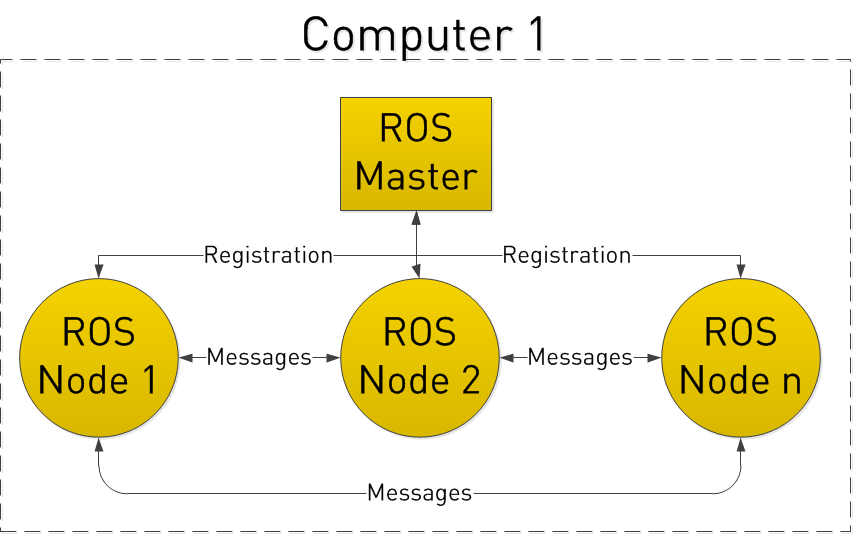
\includegraphics[scale=0.25]{ros_graph.png}
    \caption{ROS architecture overview}
    \label{fig:ros_concepts}
\end{figure}
\section{Interface between ROS and the radar}
Texas Instruments provides a ros package that interfaces radar data to the ROS message format. The incoming radar data from the mmWave EVM is decoded in oreder to create a PointCloud2 type ROS message which is published in topic \textbf{/radar/RScan}.

\subsection{PointCloud2 radar data stucture}

%%PUT figure:
The published ROS message PointCloud2 follows the mmwave demo structure (Fig. 2). Each point has 6 fields:
\begin{itemize}
\item x - position x of the detected  object in the frame of the radar.
\item y - position y.
\item z - position z (for 2D devices this is equal to zero).
\item range - range of the object relative to the radar frame.
\item doppler - radial velocity of the object relative to the radar frame.
% POR IMAGEM
\item intensity - relative power of the received signal corresponding to that object.
\end{itemize}

\begin{figure}[!htb]
    \centering
    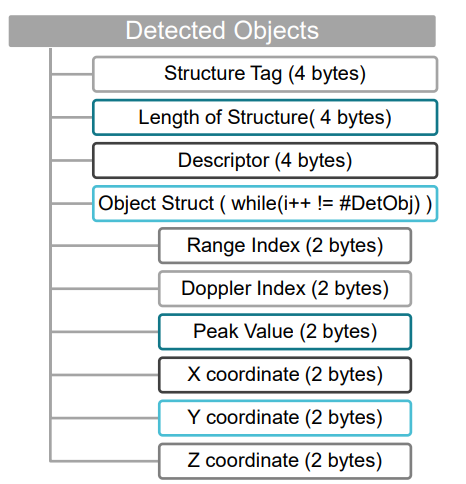
\includegraphics[scale=0.5]{2_demo_vis_struct.PNG}
    \caption{Part of the mmwave demo packet containing object detection information. This fields will be used to construct the ROS PointCloud2.}
    \label{fig:my_label}
\end{figure}
\subsubsection{Running the driver and visualizing the outputted PointCloud2}
We can visualize the published PointCloud2 message using rviz by following this steps:
\begin{enumerate}
    \item Create your ROS workspace.
    %??? Anexo
    \item Install the serial ROS package and TI mmWave ROS Driver in that workspace.
    %??? Anexo
    \item  Finnaly, while in your workspace directory run the commands:
    \begin{lstlisting}[language=bash]
source devel/setup.bash
roslaunch ti_mmwave_rospkg rviz_1642_2d.launch
\end{lstlisting}
\end{enumerate}
This will launch the TI mmWave ROS Driver nodes that configure the EVM and publish the radar data. After that rviz will load and you should be able to visualize the objects detected by the radar. Figure \ref{fig:radar_rviz} shows an example of the radar data displayed on rviz. The points correspond to object detected by the radar.
\begin{figure}[!htb]
    \centering
    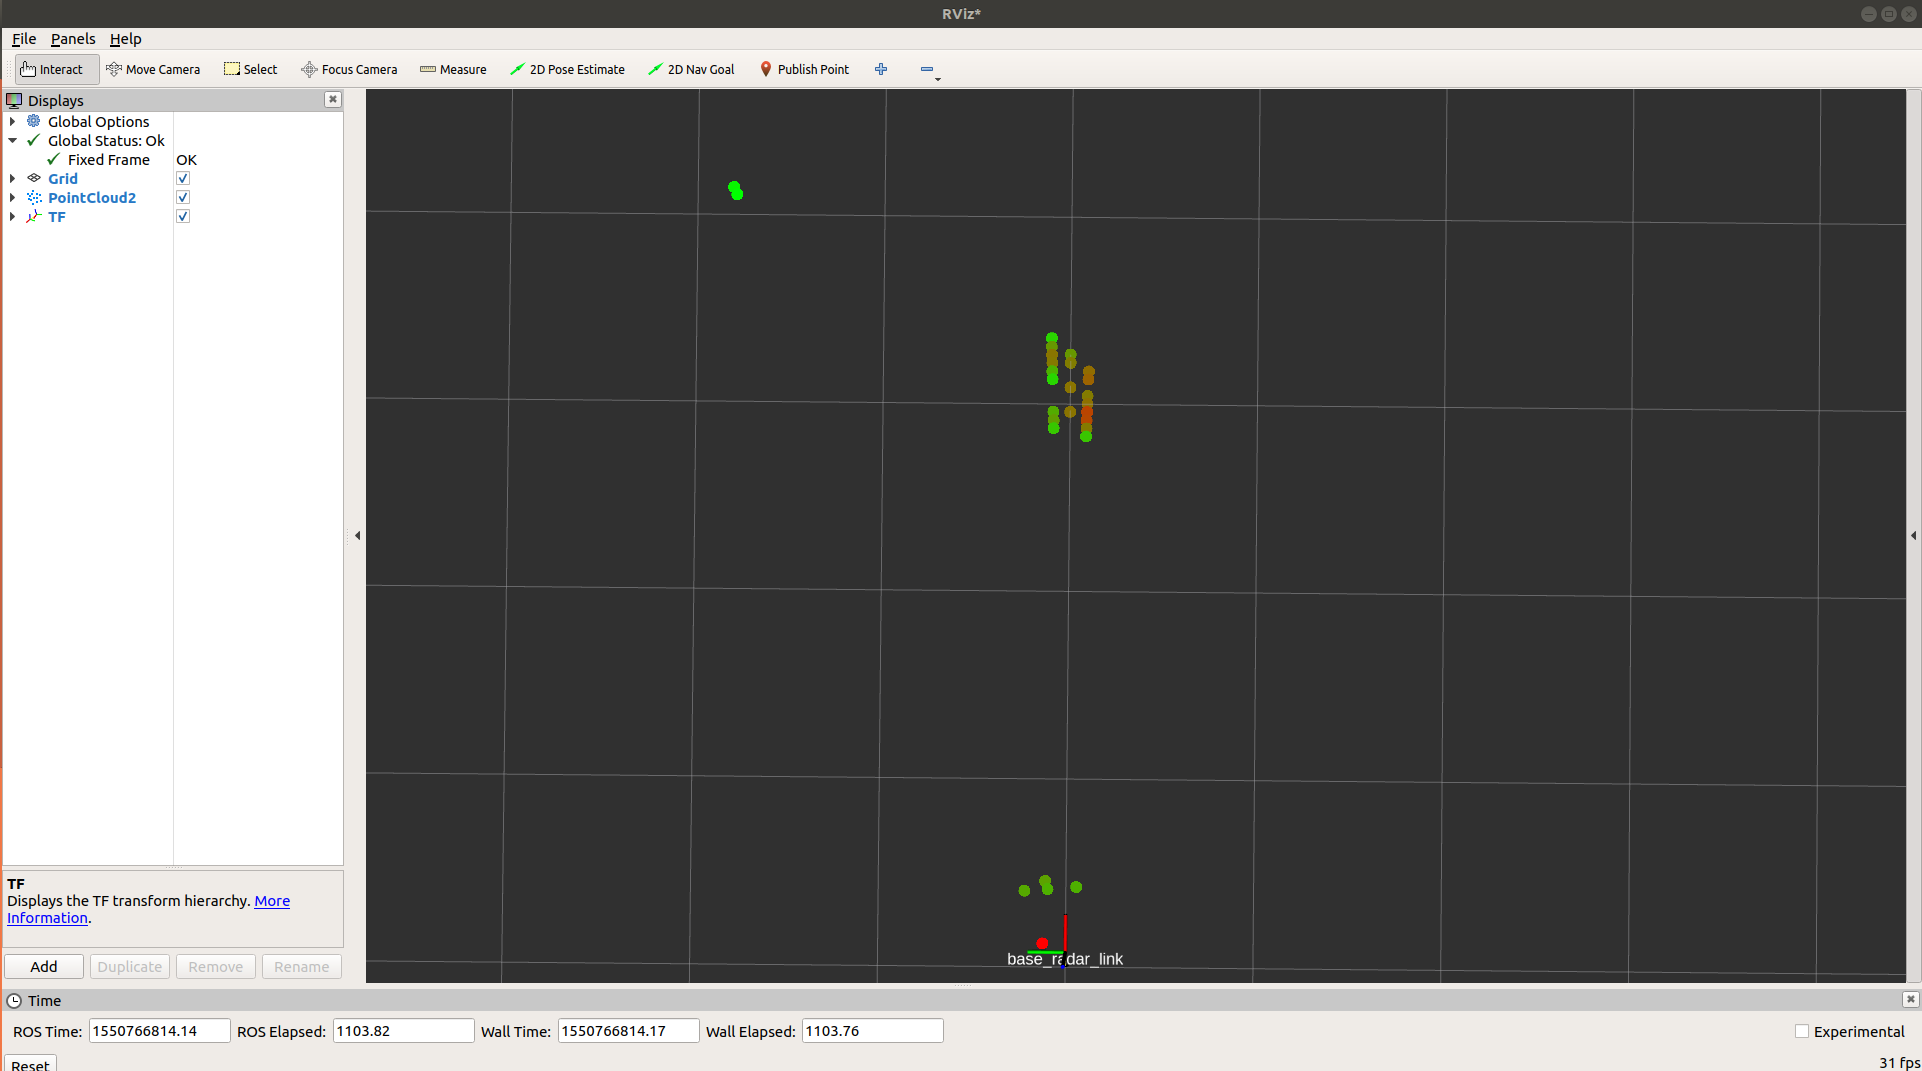
\includegraphics[scale=0.2]{pc_not_filt.png}
    \caption{Pointcloud2 radar data displayed by rviz}
    \label{fig:radar_rviz}
\end{figure}
\subsection{Visualization of the radar point cloud}
Plotting the points in the XY space plane is not enough to fully visualize the radar data sent since each point also gives velocity and intensity information.
We can visualize it by using markers such as arrows or text in rviz.
Figure \ref{fig:doppler_marker} displays the radial velocity of each point with an arrow. The size of the arrow indicates how fast the object is going. Figure \ref{fig:intensity_marker} shows the intensity values of each object in text. This type of visualization will be useful later on when we try to filter the cloud.

\begin{figure}[!htb]
    \centering
    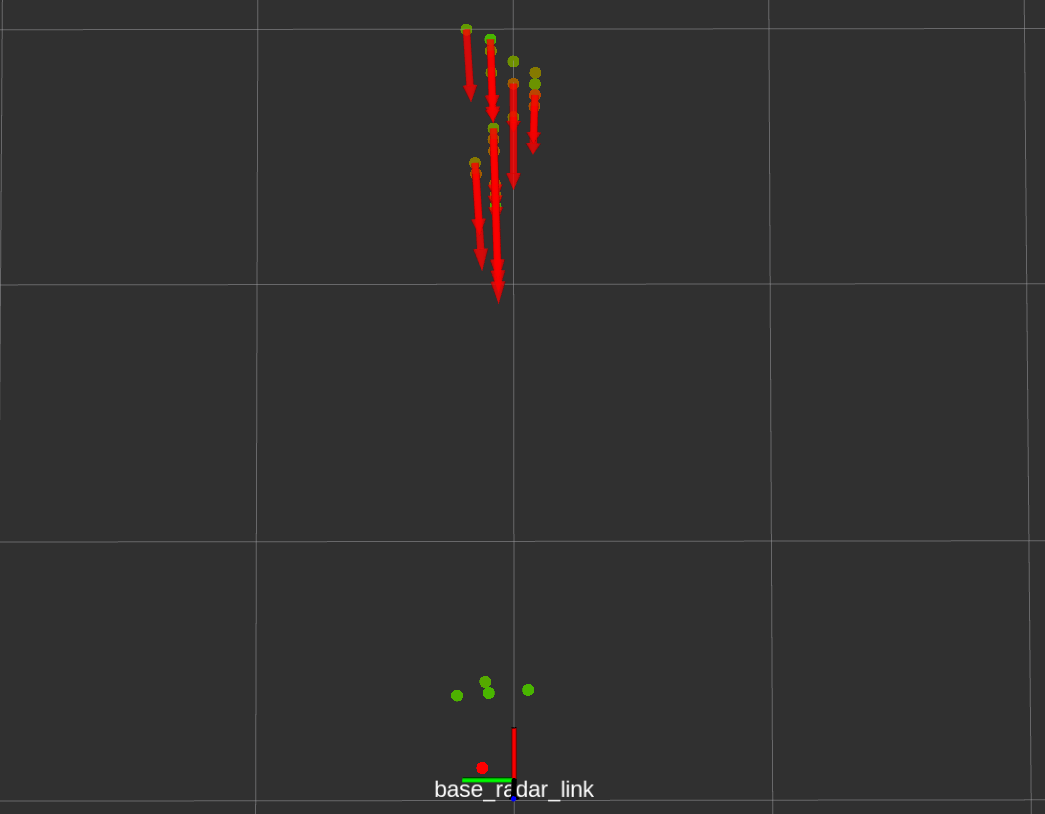
\includegraphics[scale=0.25]{doppler_marker.png}
    \caption{Arrow markers displaying the points radial velocity}
    \label{fig:doppler_marker}
\end{figure}

\begin{figure}[!htb]
    \centering
    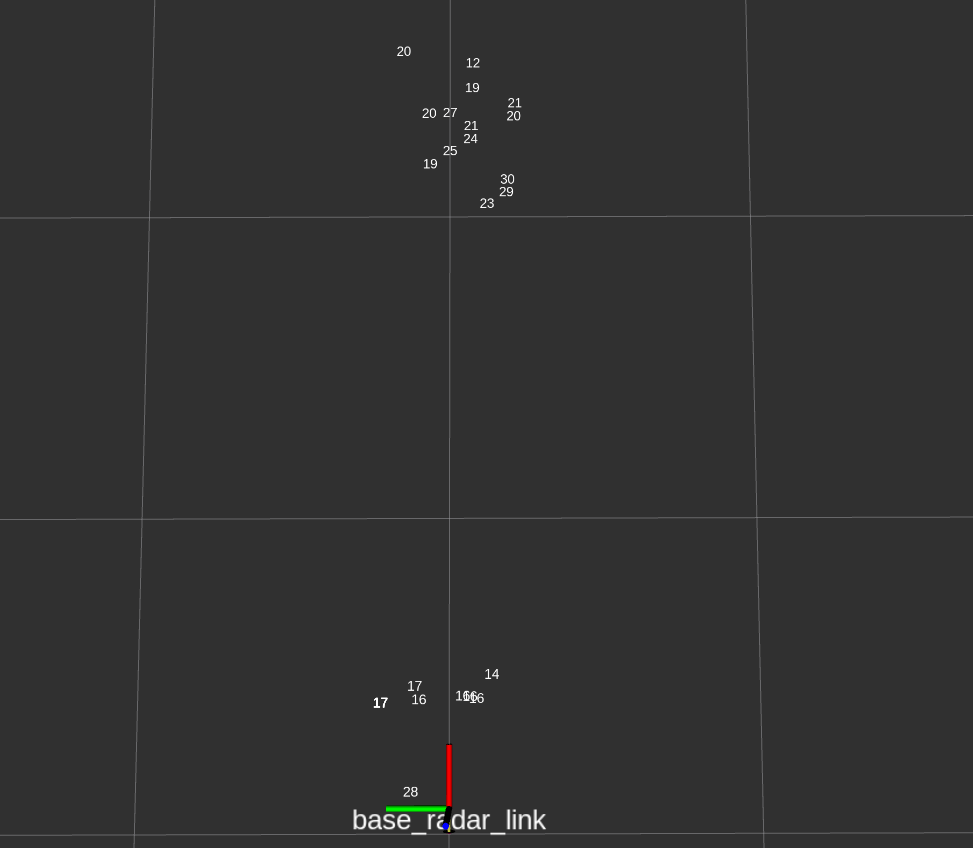
\includegraphics[scale=0.25]{intensity_marker.png}
    \caption{Text markers displaying the points intensity values}
    \label{fig:intensity_marker}
\end{figure}
\subsection{Chirp profile configuration file}
The characteristics of this point cloud such as publishing rate, range resolution, maximum range, velocity resolution, maximum velocity depends on the chirp profile configuration file loaded in the EVM. This file is located in the \textbf{"cfg"} folder of the ti mmwave package and can be replaced in order to accommodate a given application.

The easiest way to create a chirp configuration file is the mmWave Demo Visualizer. This will auto generate a configuration file given a set of specifications.
Another way of doing this is manually. This however requires the understanding of the radar operating principle and the meaning of the commands in the configuration file.
%??????????????
For more information on this topics we suggest the reading of the links bellow:
%SDK USER GUIDE
%CHIRP PARAMETER CONFIG

\section{Radar Data Processing}
Now that we have the radar constantly giving us a point cloud we can further process using the \textbf{Point Cloud Library}. PCL offers a wide variety of modules to handle point clouds. In our case we will use it for filtering, clustering and other operations.
%PCL NO FIM
\subsection{Passthrough Filters}
In the point cloud there may be some points that have undesirable characteristics, such as points with low intensity  that lead to false detections or outside of the radar operating range. To remove this points we use \textbf{passthrough filters} that specify the range of values a given field can have in order for a point to be kept in the point cloud. 

For example, if we are only interested in obstacles that are moving between 0.5 m/s and 1.0 m/s (radial velocity), this can be done by using a pass through filter on the doppler channel.
Figure \ref{fig:filters} shows an example where we delete false detections close to the radar by filtering the pointcloud by intensity.
\begin{figure}[h]%
    \centering
    \subfloat[Non filtered pointcloud]{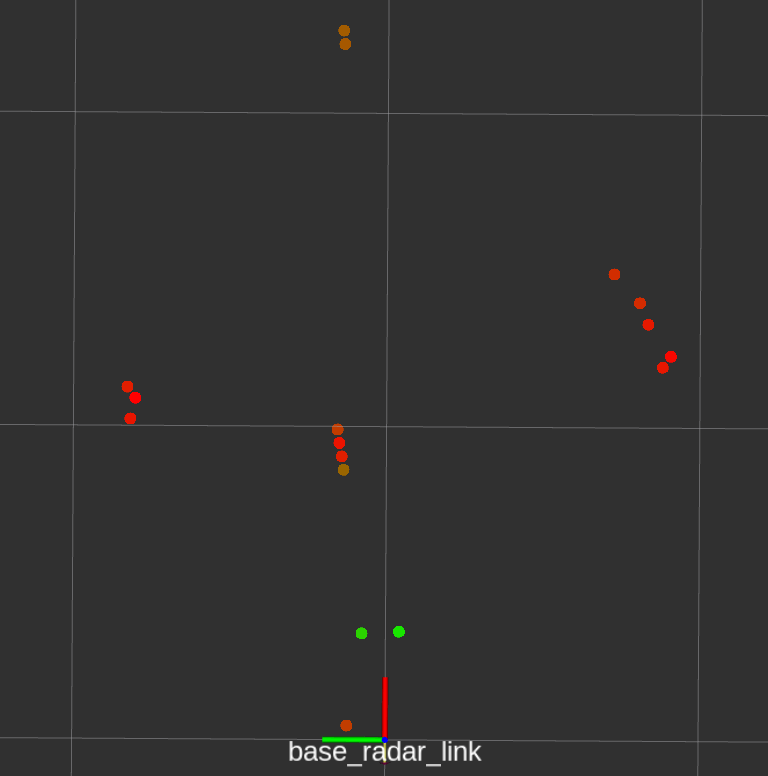
\includegraphics[width=6.34cm]{not_filt.png} }%
    \qquad
    \subfloat[Filtered pointcloud by intensity]{{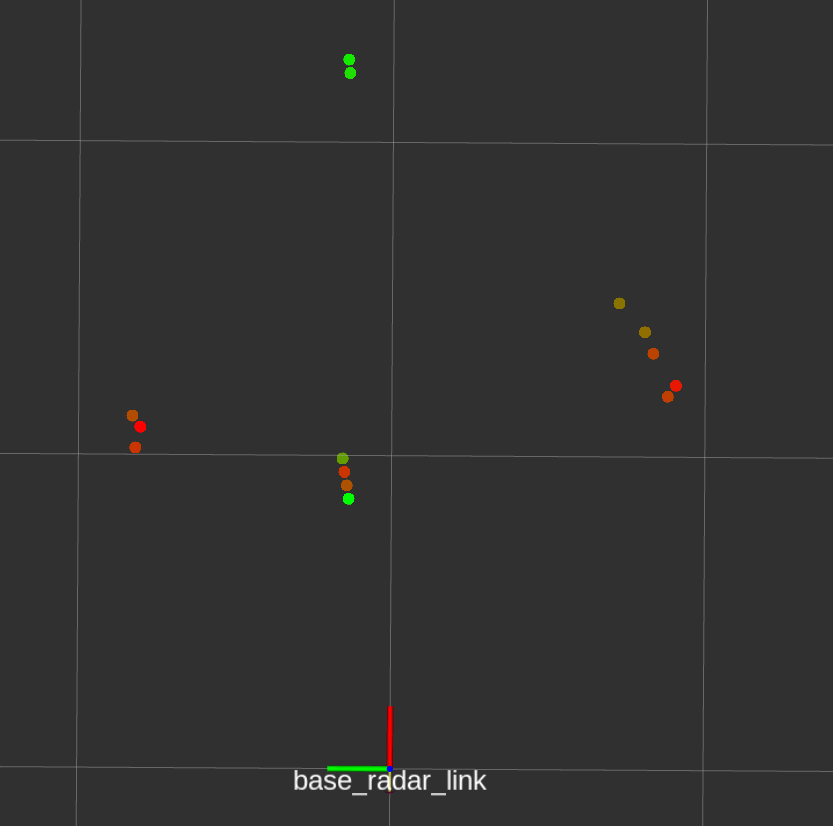
\includegraphics[width=6.34cm]{filt.png}}}%
    \caption{Example of filtering the pointcloud}%
    \label{fig:filters}
\end{figure}

%%PUT IMAGE INTENSITY FILTERING  RVIZ
\subsection{Euclidean Clustering}
%Objectivos do clustering
To identify objects such as persons we can use euclidean clustering. This identifies a subset of points that are close together. The two main parameters in this operation are:
\begin{itemize}
\item \textbf{minClusterSize} - Minimum number of points a cluster must have in order to be valid.
\item \textbf{ClusterTolerance}  - Maximum distance a point may have to a cluster member to also be counted as member of that cluster.
\end{itemize}
%%%PUT CLUSTER RVIZ FIGURE
This parameters must be tuned to the type of cluster we want to find. 
If the \textbf{ClusterTolerance} parameter is too small, it can happen that an actual object can be seen as multiple clusters, if the value is high, it could happen that multiple objects are seen as one cluster.
%In figure \ref{fig:filters} we use the module pcl
%% CLUSTER FIGURE
\begin{figure}[!htb]
    \centering
    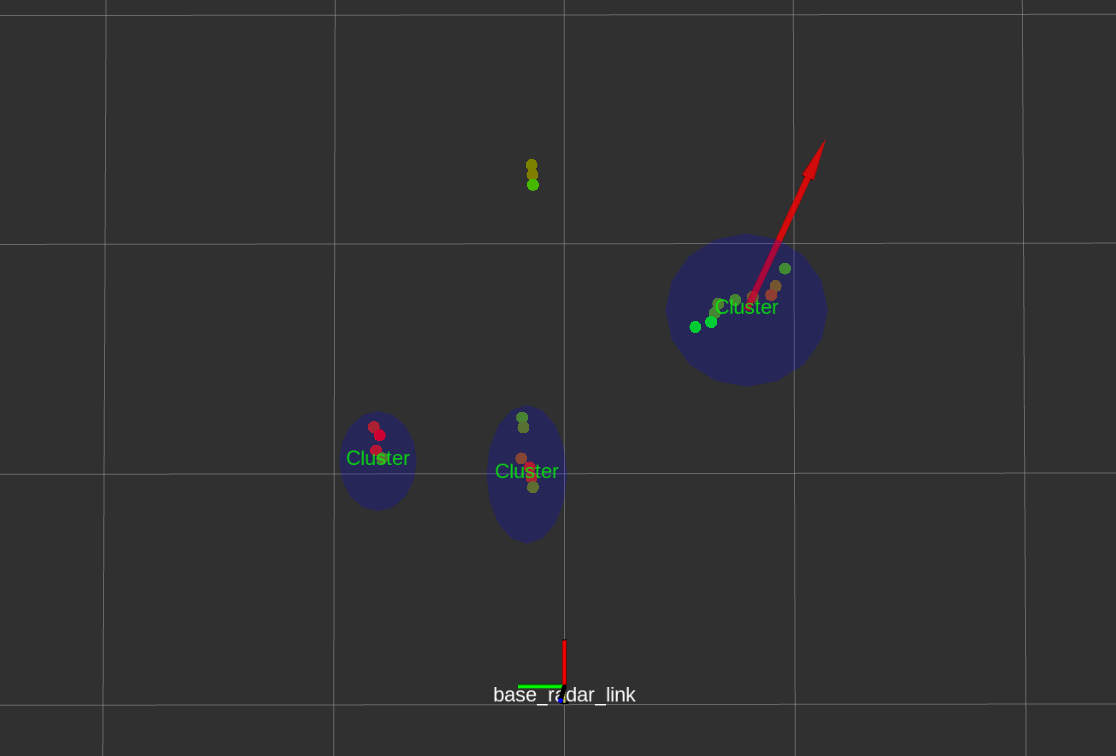
\includegraphics[width=\linewidth]{cluster.png}
    \caption{Clustering}
    \label{fig:clustering}
\end{figure}
\subsection{Using radar velocity information to predict cluster movement}
We previously said that our point cloud has a doppler channel that retrieves the relative radial velocity of the point in respect to the radar. We can use this information to compute the mean velocity of a cluster and make a prediction of its position in the future. This comes with the limitation that the radar only gives us radial velocity so the prediction will just estimate if the cluster will be closer or further away. 
However this information might be useful to avoid collisions with incoming moving objects.


%%PUT IMAGE OF PREDICTED PC2
\section{Autonomous Navigation}
%Less Implementation More general explaining of how to navigate
The ROS navigation stack is a set of software packages that properly combined can get a robot to navigate autonomously.
Figure X  shows an example of turtlebot2 using the navigation stack to drive in rviz.
However, before running it we first need to properly setup the robot.
\subsection{Requirements}
\subsubsection{Transform Configuration}
The Navigation stack requires that the relationships between the different frames must be published in \textbf{tf}, for example the transform of a sensor frame relative to the  base\_link frame. This makes it so the robot perceives what is around him correctly which is crucial in navigation.
Figure \ref{fig:tf} shows all the frames and their transforms with each other. However the main transforms we need to worry about is the sensor frames relative to the center of the robot.
\begin{figure}[!htb]
    \centering
    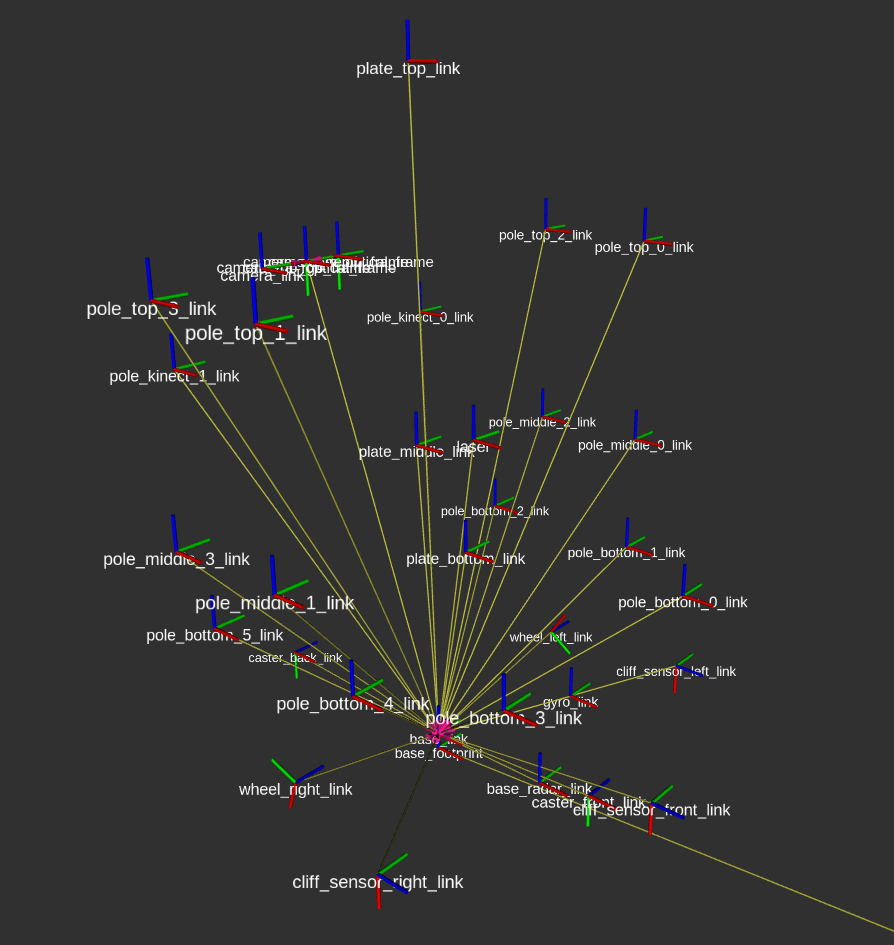
\includegraphics[scale=0.2]{tf.png}
    \caption{Transform relationships in our robot}
    \label{fig:tf}
\end{figure}
\subsubsection{Sensor sources}
To avoid obstacles we need some type of sensors that can detect them. Before running the stack we need to make sure they are publishing this information.
%in the \textbf{PointCloud2} or \textbf{LaserScan} ROS message format
In our case we will use both the \textbf{radar} (PointCloud2) and the \textbf{laser} (LaserScan) connected to our turtlebot as our observation sources.
Figure \ref{fig:sensors} shows an example of the published data from both of them in rviz.
\begin{figure}[!htb]
    \centering
    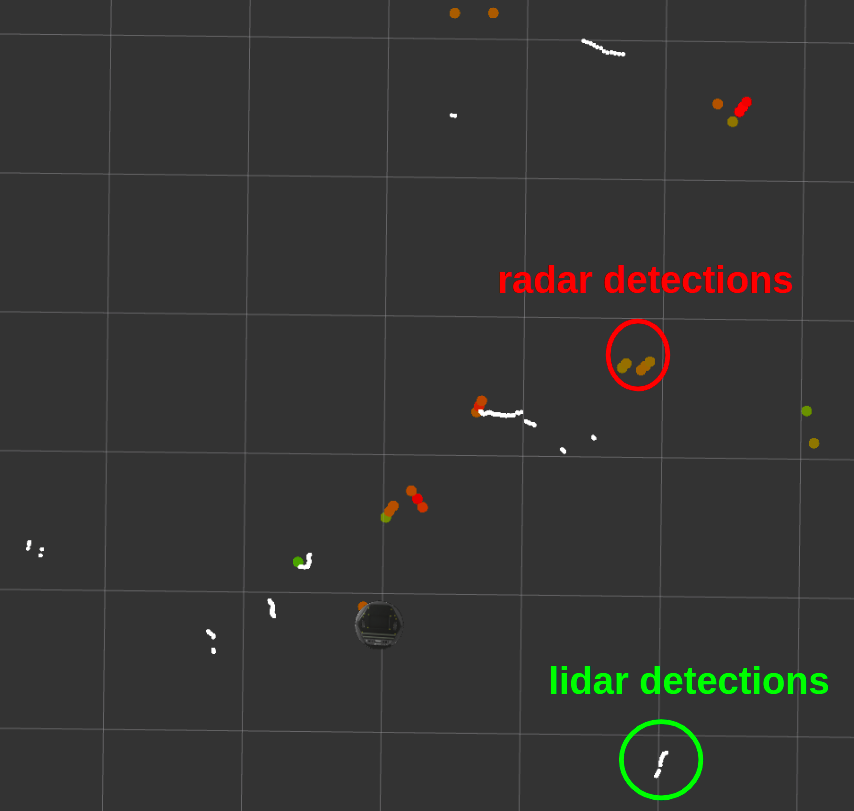
\includegraphics[scale=0.2]{sensors2.png}
    \caption{Obstacle defections by both radar and lidar}
    \label{fig:sensors}
\end{figure}
\subsubsection{Odometry}
We need to localize the robot in some way to correctly navigate. Therefore we require a topic that publishes odometry information.
%%AMCL
\subsubsection{Base Controller}
This node will subscribe to the velocity message outputted by the navigation stack and convert them into the appropriate motor commands to send to the mobile base that will actually make the robot move.

\subsubsection{Mapping}
This part is not mandatory but it helps to have a some sort of map being published to use as a global reference for the robot. Used by amcl and by the static layer of the global costmap.
\begin{figure}[!htb]
    \centering
    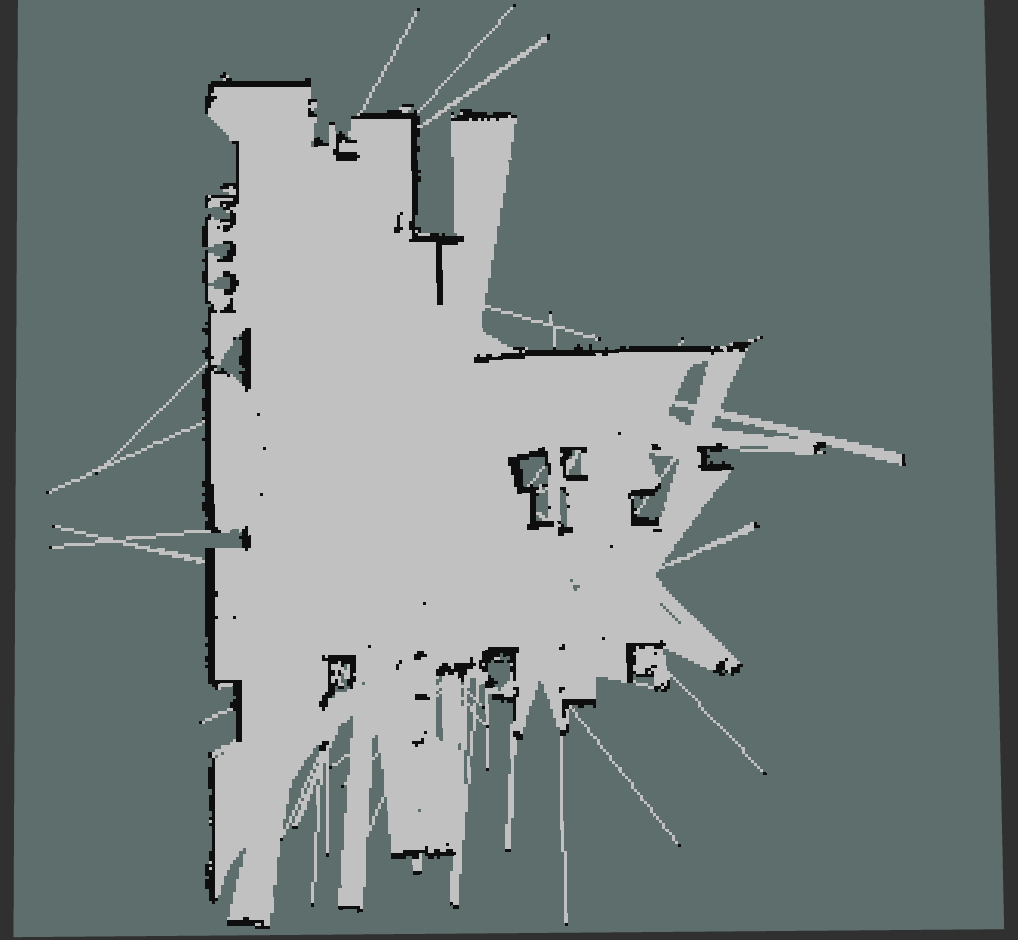
\includegraphics[scale=0.2]{map.png}
    \caption{Clustering}
    \label{fig:my_label}
\end{figure}


If the setup is done correctly we can now run the navigation stack.
\subsection{Navigation Stack components}
%%STUFF
Now that we have all the things we need for navigation we need an entity that actually processes all this information in an intelligent way to determine the best velocity command for the robot. This is done by the \textbf{move\_base node} and its peripherals.
Figure \ref{fig:plans} shows an example of the global and local plan calculated by the ROS navigation stack.
\begin{figure}[!htb]
    \centering
    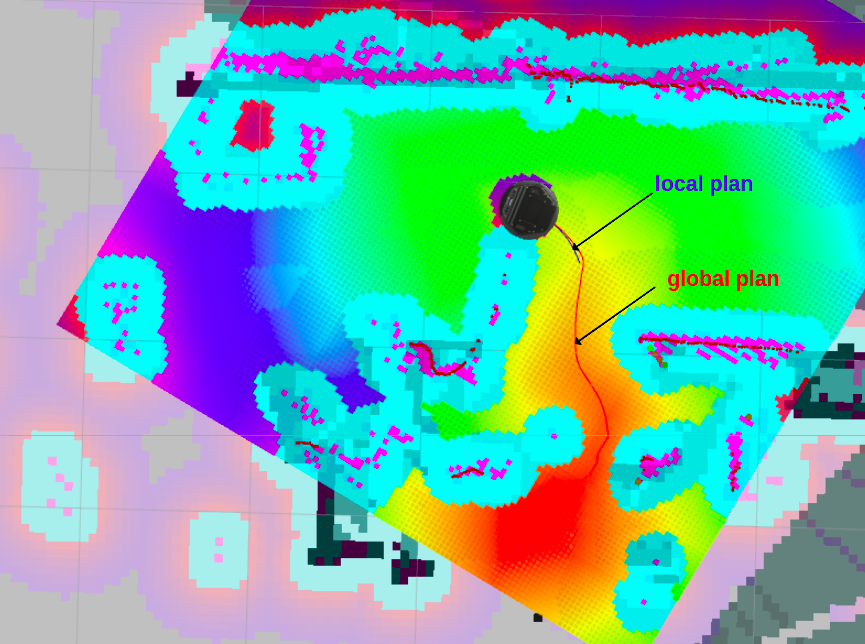
\includegraphics[width=\linewidth]{rviz_navigation2.png}
    \caption{Global and Local plan calculated by the navigation stack}
    \label{fig:plans}
\end{figure}
\subsubsection{Move Base}

The move base node base links together a global and local planner as well as a local and global costmap to achieve the end goal provided by an action server. It also loads a set of determined recovery behaviors if the planners fail to produce a valid path. 

The global and local planners are plugins specified by the user. This choice will affect the behavior of the robot depending on the planners architecture and parameters. 
%%NAV STACK IMG
\begin{figure}[!htb]
    \centering
    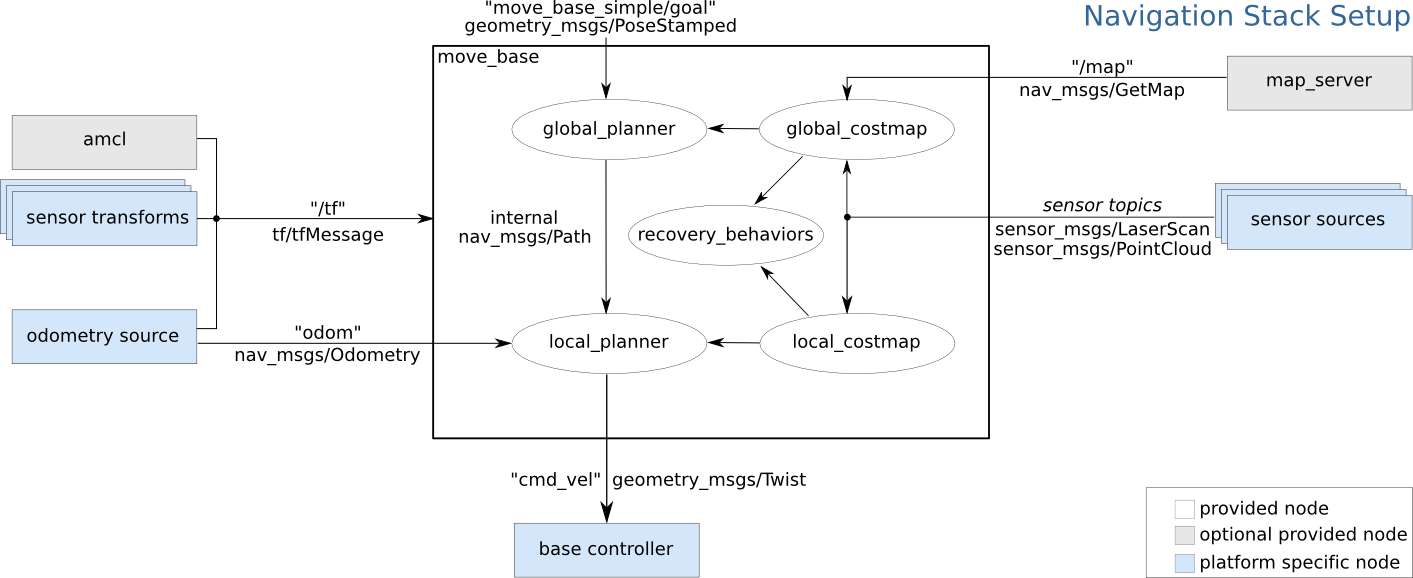
\includegraphics[width=\linewidth]{overview_tf.png}
    \caption{Clustering}
    \label{fig:my_label}
\end{figure}
\paragraph{Main Parameters}
\begin{itemize}[label={}]
    \item \textbf{Controller frequency} - Frequency at which move base will ask the local planner for velocity commands to give to the robot afterward.
    \item \textbf{Planner frequency} - Frequency at which the move base will ask the global planner for a new plan.
    \item \textbf{Planner patience} - Maximum amount of time to get a valid plan before going to recovery behavior (only if its in PLANNING state).
\end{itemize}

\subsubsection{Global Planner}
The job of this component is to produce the best trajectory for a robot to take with limited amount of information given by the global costmap. This plan can be updated when the robot gets stuck or by a user specific frequency. The algorithms used to get this path are usually \textbf{dijaktra} or \textbf{A*}. 
%%DJAKTRA AND A* global plan image
%%RVIZ image
\paragraph{Main Parameters}
\begin{itemize}[label={}]
    \item \textbf{allow unknown} - Specifies whether or not to allow the planner to create plans that traverse unknown space (global costmap defines whether or not the goal is unknown space).
    \item \textbf{default tolerance} - A tolerance on the goal point for the planner.
\end{itemize}
\subsubsection{Local Planner}
The local planner takes into account the trajectory given by the global planner and tries to follow it. However the path given may be to close to an obstacle detected and in order to avoid it we must deviate from the plan given to avoid collision. The function of the local planner is to avoid dynamic obstacles that appear while still trying to follow the global plan and goal. 

It is encharged of computing the velocity that will be sent to the mobile base. To do this it simulates various trajectories and picks the best one.

\paragraph{Getting the Best Trajectory}

The algorithm to get the best trajectory goes as follows:
\begin{enumerate}
    \item Discreetly sample the velocity space(dx and dtheta)
    \[(dx,dtheta)=(max\_velocity-min\_velocity)/nsamples)\]
    \item For each sampled velocity predict its trajectory in a given time frame (\textbf{sim\_time}).
    \item Evaluate the cost of each trajectory  by using the value cost function
    \item Pick the one with lowest cost and publish the associated velocity.
    \item Repeat for a given rate (\textbf{controller\_frequency})
\end{enumerate}
%%SIMULATION IMAGE


\paragraph{Cost Function}
The cost function used to evaluate a trajectory is given by:
\[
       cost = 
  pdist\_scale * path\_dist
  + gdist\_scale * goal\_dist
  + occdist\_scale * maxobscost 
\]
Where \textbf{path\_dist} is the distance from the endpoint of the trajectory to the global path in map cells or meters, \textbf{goal\_dist} is the distance from the endpoint of the trajectory to the local goal in map cells or meters and \textbf{maxobscost} is equal to the \textbf{maximum obstacle cost} (given by the local costmap) along the trajectory .
%%RVIZ cost cloud
\begin{figure}[!htb]
    \centering
    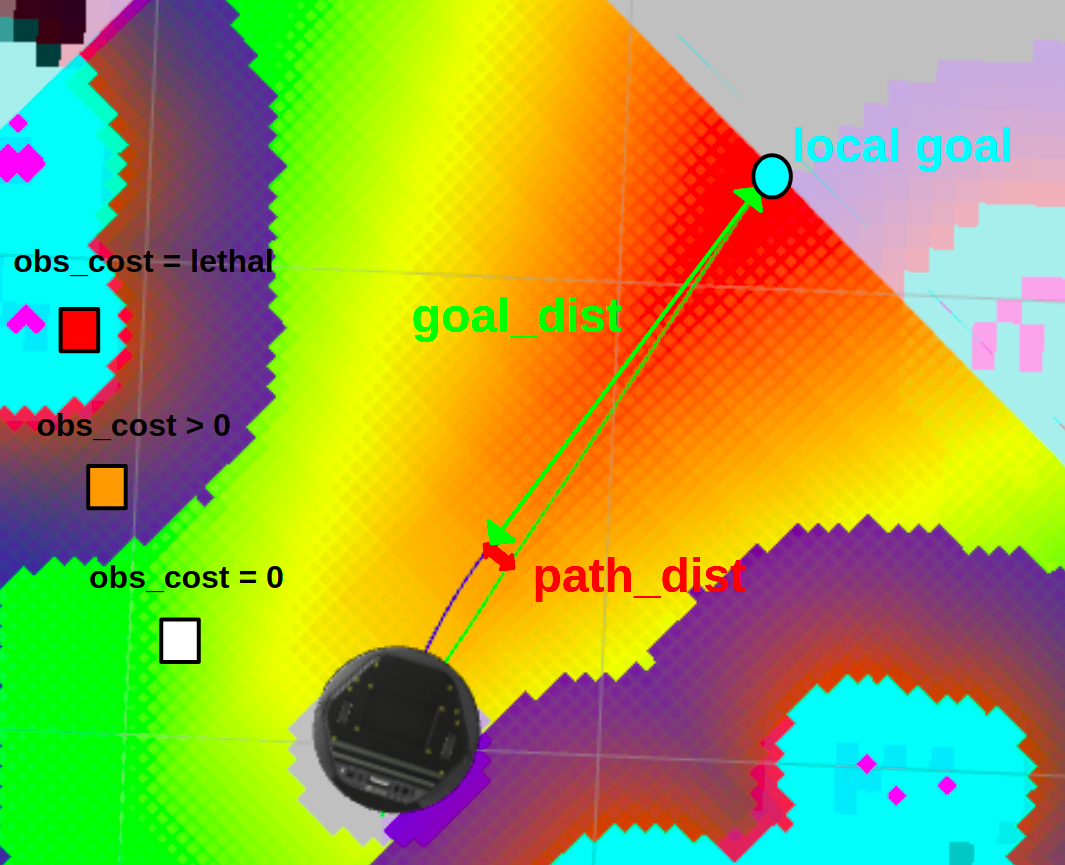
\includegraphics[scale=0.3]{cost_cloud.png}
    \caption{Cost cloud published in rviz. Red and green cells correspond to low and high cost respectively}
    \label{fig:my_label}
\end{figure}
\subsubsection{Local and Global Costmap}
The global and local costmap share the same class, the  \textit{Costmap2DROS}. This class consists of a layered costmap that takes into account various layers defined by the user.

\paragraph{Available Layers}
\begin{itemize}[label={}]
    \item \textbf{Obstacle Layer} - Marks objects retrieved from \textbf{observation\_sources} with lethal value. It also raytraces observations to clear out space.
    %Does more stuff
    \item \textbf{Inflation Layer} - Inflates the detected obstacles taking into account the \textbf{robot\_radius} and \textbf{inflation\_radius}. The closer the cells are from a lethal obstacle the more value they will have.
    %%....(needs explanation)
    \item \textbf{Static Layer} - Retrieves static information from the /map topic and marks them has lethal objects (Typically only used in global costmap). Obstacle layer may overwrite this layer if the user chooses too.
\end{itemize}
Figure \ref{fig:layers} shows how the combined layers produce the master costmap that will be used by the planners.
\begin{figure}[!htb]
    \centering
    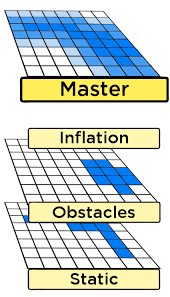
\includegraphics{layers.png}
    \caption{Different layers used to create the final costmap grid that will be used in the navigation stack}
    \label{fig:layers}
\end{figure}
All the user defined layers will in conjunction create the final master costmap that will be used by the planners.

\subsection{Results}

\begin{comment}
%%RVIZ costmap
\*
\section{Using the radar for autonomous navigation of the turtlebot}

\subsection{ROS Navigation stack setup}

The ROS navigation package offers a reliable way for a robot to navigate alone. In order to  do this it needs a sensor source to detect obstacles, a reliable source of odometry and optionally a mused . The map is used as global reference to the robot.
%%IMAGEM ROS NAVIGATION STACK
\subsubsection{ROS Navigation structure}
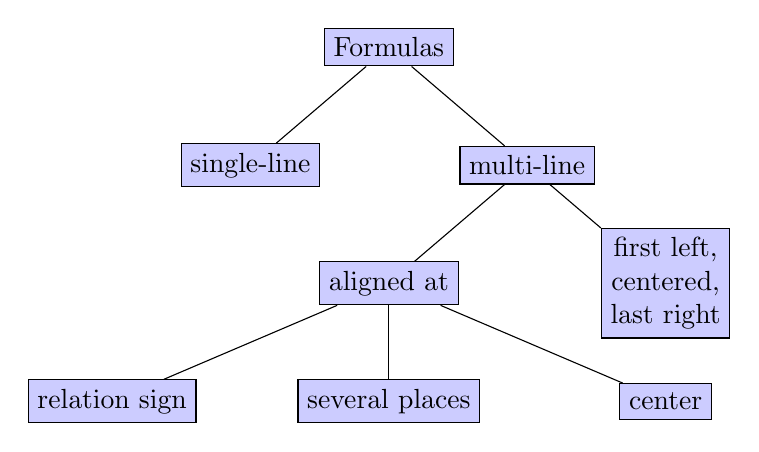
\begin{tikzpicture}[sibling distance=10em,
  every node/.style = {shape=rectangle, sharp corners,
    draw, align=center,
    top color=blue!20, bottom color=blue!20}]]
  \node {Formulas}
    child { node {single-line} }
    child { node {multi-line}
      child { node {aligned at}
        child { node {relation sign} }
        child { node {several places} }
        child { node {center} } }
      child { node {first left,\\centered,\\last right} } };
\end{tikzpicture}

In this case we will use the radar pointcloud and the lidar laserscan as sensor sources and amcl for localization.
\subsection{Results}


%RADAR CONCEPTS
\section{Radar basics}
In order to retrieve the best data for our application we first need to understand how the radar works. The following sections will try explain how the radar calculates the range, velocity and angle of an object.
\subsection{range Detection}
An FMCW radar transmits a signal called a “chirp”. A chirp is a sinusoid whose frequency  increases linearly with time.
%% put A t and f t plot
A chirp is characterized by a start frequency (fc), bandwidth(B) and duration (Tc). The slope (S) of the chirp is the rate at witch the frequency of the chirp increases and is given by:
\begin{equation}
    S=\frac{B}{T_c}
\end{equation}
%%PUT SOME TEXT
Object detection follows this steps:
\begin{enumerate}
    \item The chirp is transmitted by the TX antenna
    \item The chirp is reflected off an object and the reflected chirp is received at the RX antenna
    \item The RX signal and TX signal are ‘mixed’ and the resulting signal is called an ‘IF signal’
\end{enumerate}


%%PUT IMAGE
%%%When the transmitted chirp encounters an object it will reflect back to the radar and will be captured by the RX antenna.
The RX signal is a sum of delayed versions of the TX signal. This means that the resulting IF signal will be a combination of sinusoids. Each of this correspond to a reflection of an object. For object $i$ the corresponding frequency $f_i$ is equal to:
\begin{equation}
    f_i=S\tau_i
\end{equation}
Where $\tau_i$ is equal to the round trip delay of the wave and is equal to:
\begin{equation}
    \tau_i=\frac{2d_i}{c}
\end{equation}
Where $d_i$ corresponds to the distance of the object to the radar and $c$ the speed of light.
%% PUT image
Putting this together the distance of object $i$ is given by:
\begin{equation}
    d_i=\frac{f_ic}{2S}
\end{equation}
\subsection{range resolution}
\subsection{velocity Detection}
\subsection{angle Detection}

 %A cluster is just a subset of points of the cloud that are close together. This takes into account if a point has alot of close neighbours. If it has than it is considered a cluster.  
 \begin{figure}[!htb]
    \centering
    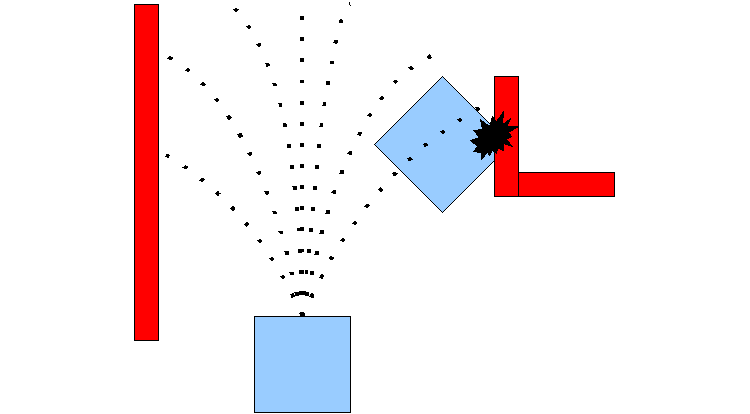
\includegraphics[width=\linewidth]{local_plan.png}
    \caption{Clustering}
    \label{fig:my_label}
\end{figure}
\end{comment}
\end{document}